\documentclass[11pt]{article}
\usepackage{amsmath,amsfonts,amssymb,float,bbm,url, graphicx}

\title{}
\author{}
\date{\today}

\graphicspath{{imgs/}}

\begin{document}

\maketitle

\begin{abstract}

\end{abstract}

\section{Introduction}


\section{Data and Methodology}
We collected 10,908,817 tweets using Twitter's Streaming API\footnote{\url{https://dev.twitter.com/}} starting from December 4th, 2013 until January 13, 2015. A bounding box (32º 25' 4.2414" N, 117° 18' 49.5066" W and 33º 5' 53.3178" N, 116º 49' 17.9142" W) was used to filter only to those messages originating from San Diego and Tijuana. Each tweet consisted of a unique identifier, date-time of submission, coordinates of submission (i.e., latitude and longitude), language of submission, and the message itself. Even though this process comes with the limitation that we only have access to approximately 1\% of all the tweets \cite{Olteanu2015}, previous work have shown that the data obtained from the API closely resembles a random sample drawn from the full Twitter stream \cite{DBLP:journals/corr/MorstatterPLC13}.

Each tweet was preprocessed in the following way: (i) all characters were lowercased; (ii) URLs and mentions were replaced with placeholders \_\_URL\_\_ and \_\_MENTION\_\_ receptively; (iii) Four-digit numbers were replaced by \_\_4NUM\_\_, any other length number was replaced by \_\_NUM\_\_, (iv) Every punctuation character  was removed except for @,\#,\_ and newlines; (v) negations were handled by marking all tokens up to the next punctuation. Tweets were grouped according to their submission language. This resulted in two datasets, one for English ($12,212,416$ tweets) and one in Spanish ($764,709$ tweets). 

\subsection{Obtaining country of submission}
In order to find the country of submission from the GPS coordinates, we trained a Gradient Boosting Classifier (GBM). GBM is a random forest ensemble method based on the decisions of weak tree classifiers. This method has been shown to produce good results for most problems \cite{JMLR:v15:delgado14a}. We trained our classifier on $2838$ coordinates-country pairs obtained from the GeoNames Gazetteer\footnote{\url{http://www.geonames.org}}. Our model was trained to classify latitude and longitude into country names with options between U.S., M.X., and Other. We tested the model's accuracy in a held-out test set of $500$ samples obtaining 99.18\% accuracy.

\subsection{Extracting sentiment}
The sentiment analysis method used was a simplistic variation of the SAIL method, presented in \cite{malandrakis_sail_2014} for the SEMEVAL 2014 Challenge. In its original implementation, it is a method that derives lexicon features that describe the emotion of a text through a multitude of statistics. 

\subsubsection{Expanding dictionaries}
To obtain comparable metrics between languages, we decided on using an emotional lexicon that was available in both English and Spanish. One of such corpora is Affective Norms for English Words (ANEW) \cite{bradley1999affective} and its Spanish couterpart ANSW \cite{redondo2007spanish}. Both of these provide ratings for $1035$ words in a valence, arousal and dominance scale. Additionally, they provide with a frequency statistic of how many times a word appeared. Unfortunately, taken as it is, most of these words won't appear in a regular tweet. In order to expand the coverage of our dictionaries we decided on the following method:

\begin{enumerate}
	\item Learn a domain-specific similarity model between English (Spanish) words.
	\item For each word $w$ in ANEW (ANSW):
	\begin{enumerate}
	 	\item Find $n$ similar words in the domain and their similarity ratings.
	 	\item For each similar word $s$ with similarity rating $\eta_s > \tau$: \\
	 		  Asign a valence and arousal rating as follows:
		 		\[ valence(s) = valence(w) * \eta_s	\]
		 		\[ arousal(s) = arousal(w) * \eta_s	\]
	 \end{enumerate} 
\end{enumerate}

We assume that similar words must have similar valence and arousal ratings, and that this similarity is mediated by the cosine score. Our domain-specific similarity model was learned using 400 dimension Word2Vec \cite{mikolov2013distributed} on $12,212,416$ tweets for English and $10,522,314$ for Spanish. We set $n$ to be 100 and the threshold $\tau$ to $0.5$. The resulting expanded ANEW dictionary had $10,075$ (ANSW, $11,200$) words. 

 % For example, the ANEW word ``violent'' has a valence rating of $(\mu =2.29, \sigma=1.78)$. The most related words to the word violence, as seen in Twitter data, were: ``nonviolent'' ($\eta_s = 0.52$), ``hateful'' ($\eta_s=0.51$), ``immoral''($\eta_s = 0.50$), ``civilized'' ($\eta_s=0.49$), ``harassment'' ($\eta_s = 0.49$). 

\subsubsection{Calculating sentiment of a tweet}
In order to obtain a tweet-level sentiment, we did the following: (i) find the words in the tweet that are in the expanded ANEW (ANSW) dictionary; (ii) If the tweet has 1 or less words in the dictionary, classify it as a neutral sentiment; (iii) Else, statistically average the word's valence and arousal. Our statistical average function was a weighted average, using the frequency of a word as the weight of that emotion. Thus a word that was seen $100$ times in ANEW carries the double emotion than one only seen $50$ times. 

\section{Results}
\subsection{By Language}
We obtained arousal and valence ratings for all the tweets. One out of every four tweets ($24.498\%$) in English had two or more words with emotion (i.e., found in the expanded ANEW dictionary). In contrast, only $12.923\%$ had two or more words in the Spanish expanded dictionary. Figure \ref{fig:distrEmolang} shows the distribution of number of dictionary words found in the tweets according to their language. There was no significant difference in the distributions of emotional words in tweets (KS-test, $p > 0.05$)

\begin{figure}[tb]
	\centering
	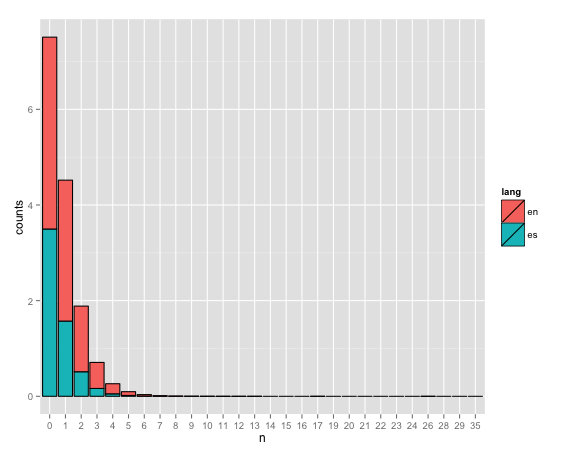
\includegraphics[scale=.6]{distr_Emotion_lang}
	\caption{Distribution of words found in ANEW and ANSW}
	\label{fig:distrEmolang}
\end{figure}

\subsubsection{By Geography}

\section{Conclusion}

\bibliographystyle{plain}
\bibliography{references}


\end{document}